\chapter{Methodology}\label{chapter:Methodology}
The following part explains the single steps of the forecasting process for this Interdisciplinary Project in detail.The forecast will be presented from the very beginning.\newline
First of all, the problem will be defined properly. Then the information needed will be specified and gathered. This data is then analyzed in a preliminary step and after this models for the data will be examined. In the end the result of the models will be evaluated and further proceeding will be explained in the final conclusion.
\section{Problem Definition}\label{section:Problem Definition}
Before the forecasting can start, some general questions have to be solved. Most important is the question of who is requesting the forecast and what will the forecast be used for. In order to acquire this information, the COO, Emanuel Pallua, who is requesting this forecast, is interviewed. The aim is to forecast the preparation time of a restaurant. This is needed to be able to send the driver to the restaurant just in time when the meal is prepared. This improves the algorithm and reduces driver idle times. The forecast should be done once to be evaluated and later the most accurate method should be integrated into the algorithm itself for automatization. In addition to this, Sebastian Sondheimer gave some input regarding the forecast parameters. The forecast should include different periods, like the current time, day and a limit time of the past. This will be explained in more detail later.\newline
After having the requirements from business side, the tech side is examined. Sergej Krauze, CTO and responsible for the algorithm, explained that the algorithm takes all restaurants with open orders, the customers and the drivers to calculate the most efficient route to pickup and delivery the food. The algorithm is written in Java so it would be welcome to develop the forecasting in Java as well. Finally Stefan Rothlehner, CTO and responsible for the backend, had to be questioned, what data is available and how it can be extracted. Every order is stored in a PostgreSQL database on heroku, on which it can be accessed and downloaded.
\section{Gathering Information}\label{section:Gathering Information}
The database is dumped at two dates in time. The training data set was downloaded at the 26th of March 2015 to create a forecast which later can be compared to a test data set. This test data set was extracted from the server on the 29th of April. Speaking in number of orders, the csv file of the first extraction has 3034 entries while the second one has 4973 entries. In addition to the historic data, the operations team was interviewed for their personal experience with the preparation times. They said that estimating around 15 minutes is more or less accurate except for some restaurants which are known to take much longer.\newline
This information is valuable since the historical data has some weaknesses. The biggest problem is the size of the gathered data. Forecasts need big amounts of information to generate a meaningful result so the data.\newline
In order to use the datasets from the csv files, it has to be parsed into objects in the Java program. For this purpose a csv parser library is used. The library reads the csv file and matches the orders from the database to the OrderModel.class of the code. Not all attributes of the database are used, only the one related to the forecast are picked from the information. Since there is no tracking in the restaurant for the preparation time, it was decided to take the time interval from the point in time at which the restaurant knows from the order until the driver leaves the restaurant. In the process of volo, the printer in the restaurant prints the recipe at the same time the driver accepts the delivery, which is saved in the database as \texttt{"accepted\_at"}. The timestamp of the driver leaving the restaurant is saved in \texttt{"delivery\_started\_at"}. Since it is not the task to figure out the exact the preparation time but the time from when the order is send to the restaurant and when the driver can picks it up, there are no modification to the time done.
\section{Preliminary Analysis}\label{section:Preliminary Analysis}
The weather or season can also affect the preparation time. There can be seasonal cycles or trends caused by rising brand awareness. All these different situations have to be taken into account. There can also occur other factors, like marketing campaigns, but this has not happened in the recorded time frame. In order to discover these patterns and get a feeling for the data, a preliminary analysis is done.
\subsection{Raw Data Cleanup}\label{subsection:Raw Data Cleanup}
First of all the average preparation time of the orders is calculated. This is done to get a feeling in which how long the restaurants usually take. It can give a rough estimation of what can be expected and compared to the forecast later to find out whether the result is total unrealistic or pretty close to what is possible. In addition to the average time, a visualization of the data is done. The best way to do this is to use a time series plot. In the graph it is very easy to see anomalies and patterns.\newline
The average time and the visualized raw data is shown and explained below.

\begin{figure}[h]
\begin{center}
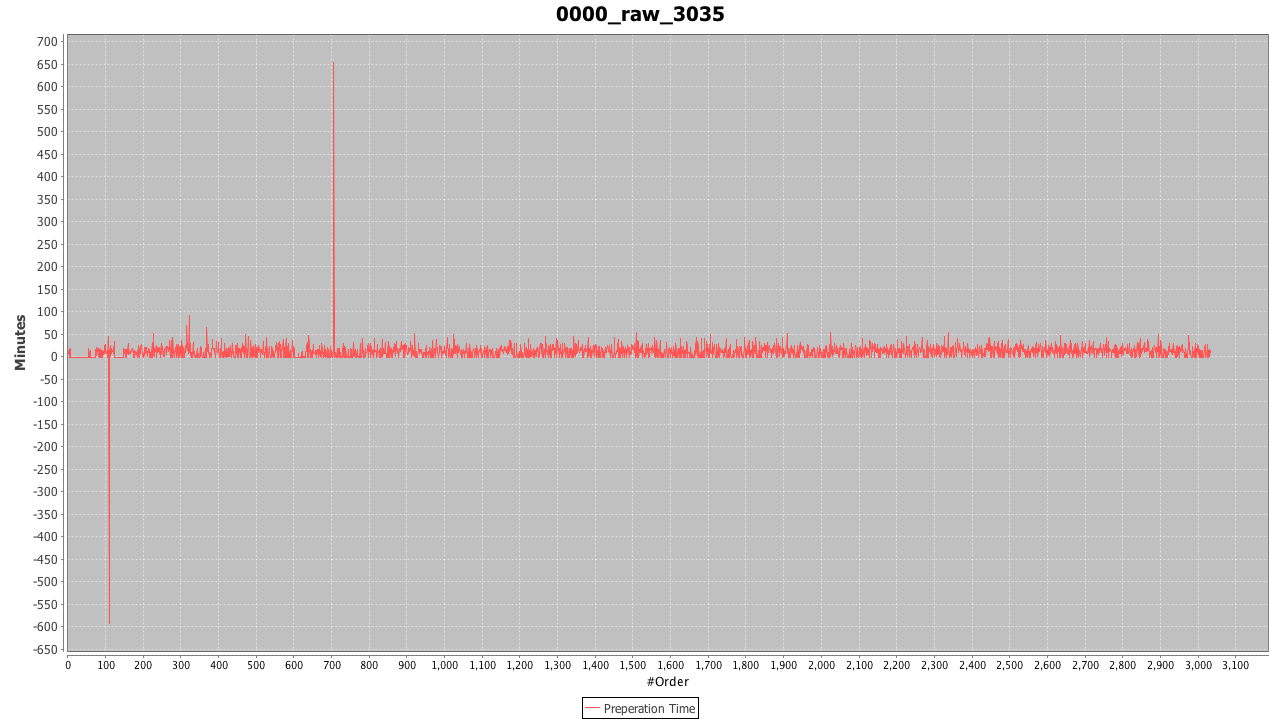
\includegraphics[width=10cm]{images/0000_raw_3035.png}
\caption{An example figure}
\label{fig:example}
\end{center}
\end{figure}

The analysis of the diagram reveals the first problems of the data. The orders from the trainings dataset still contain unfinished orders, bugged orders, which were finished at a wrong point in time, and orders which have corrupted time stamps. Unfinished orders have missing timestamps and like unreadable timestamps they get as "total"-time attribute -1 to be detectable. This can be observed in many cases in the diagram above. Also an order which was finished the next day can be seen around the 100 mark. This flaws in the data lead to a result of 12 minutes of average preparation time. This cannot be taken as a serious results since the -1 results lower the average drastically below of what the real average would be like. These values have no value to the forecast and have to be removed from the pool. This is done by removing all -1 from the used data. The result can be seen in [] below. This increases the average preparation time to 16 minutes. This can be explained because of the missing -1 values.

\begin{figure}[h]
\begin{center}
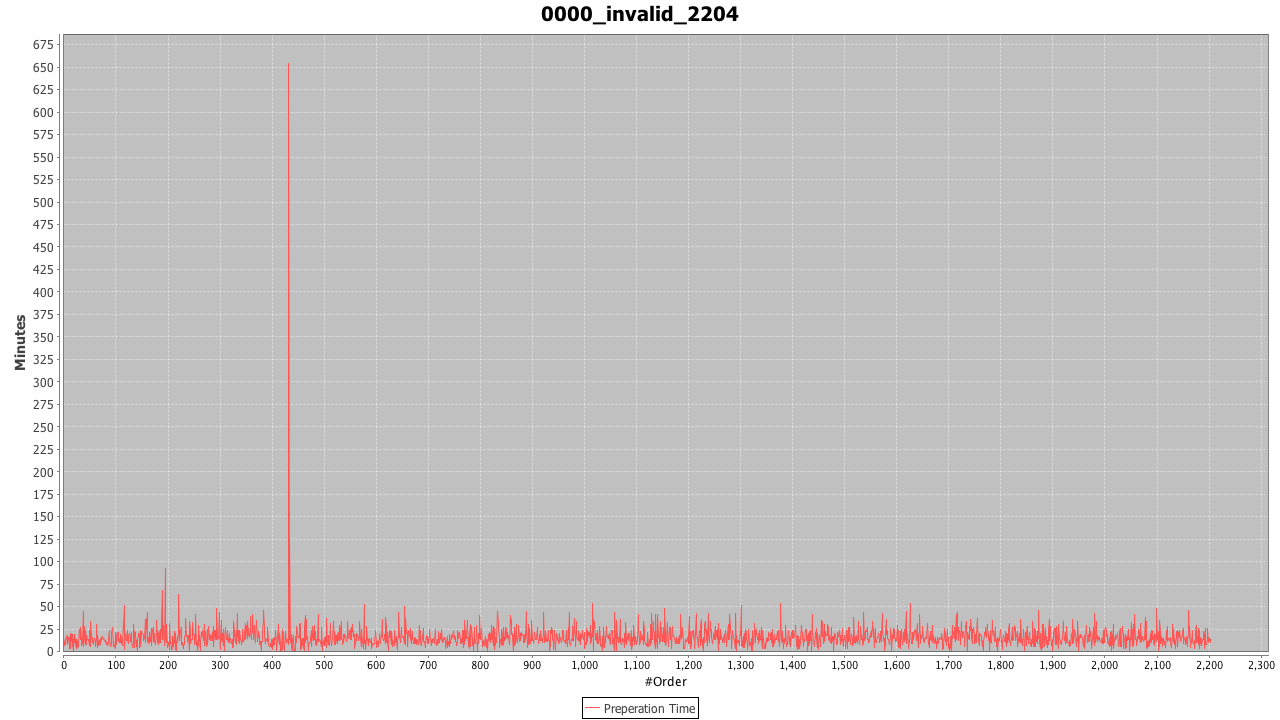
\includegraphics[width=10cm]{images/0000_invalid_2204.png}
\caption{An example figure}
\label{fig:example}
\end{center}
\end{figure}

After removing the obviously unusable orders, the ones which were finished long time after completing the delivery, mostly because of bugged software, have to be removed. For this purpose the Grubbs training for outliers is applied to the dataset and all values seem not to come from a normally distributed population are removed. This results in an average preparation time of 15 minutes which is the same result as the operations team suggest to use as a basis.

\begin{figure}[h]
\begin{center}
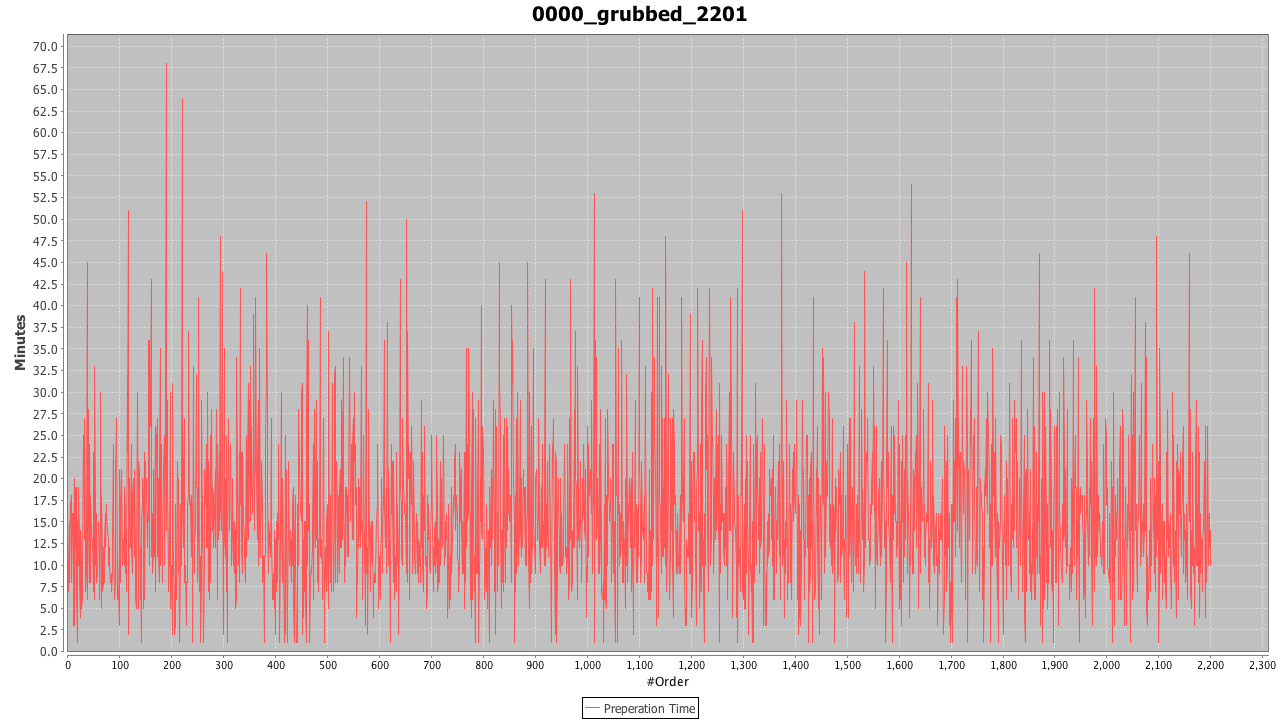
\includegraphics[width=10cm]{images/0000_grubbed_2201.png}
\caption{An example figure}
\label{fig:example}
\end{center}
\end{figure}

Now the usable training dataset is extracted from the input data, we can analyze it for patterns for patterns or similarities.\newline
\texttt{0000\_grubbed} is very fine and sorted by order. It was created to get an overview focused on orders and does not have a time component. It cannot provide information about patterns since patterns rely in this case on time. In order to include this, the orders are sorted by day and put into a time plot [].

\begin{figure}[h]
\begin{center}
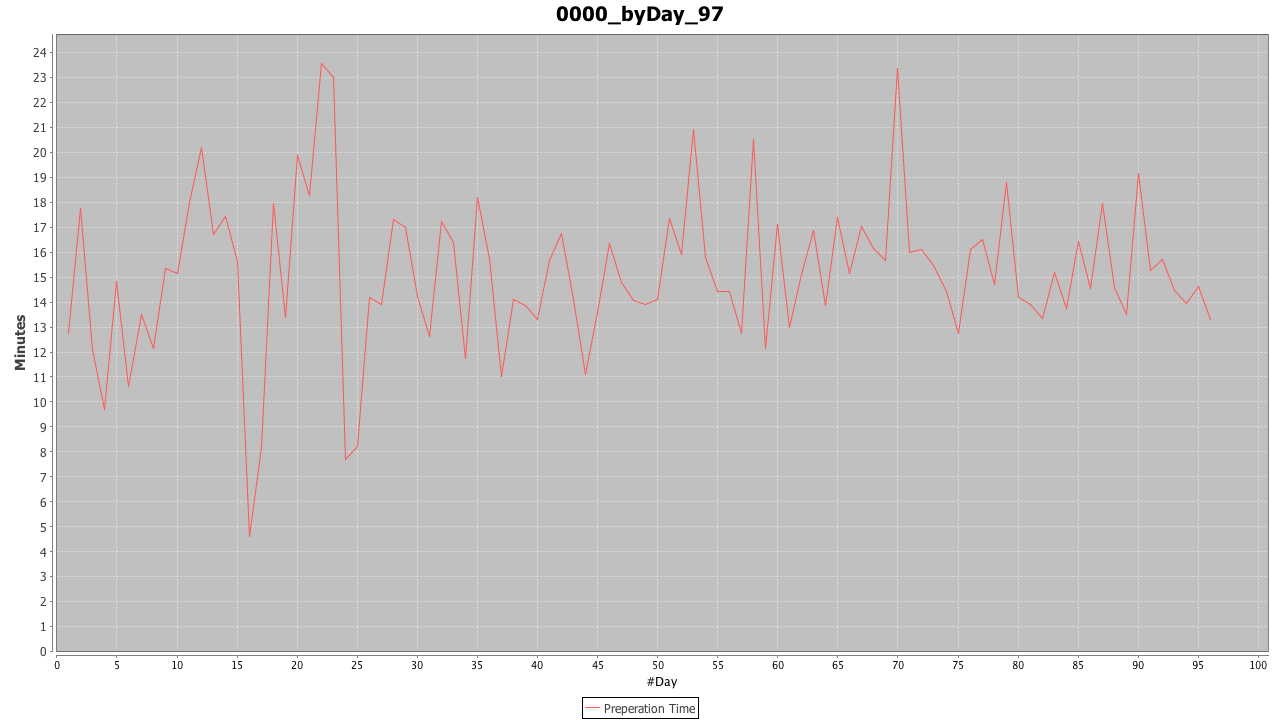
\includegraphics[width=10cm]{images/0000_byDay_97.png}
\caption{An example figure}
\label{fig:example}
\end{center}
\end{figure}

Since no clear trend or pattern can be observed in a day by day analysis, a box and whisker diagram is created from the data. It shows the median and average preparation time as line and point inside the box. The box represents the upper and lower quartile of preparation times in which 50 \% of the data is while the red whiskers visualize the area without outliers, which are red circles and a red triangle in case they are out of scale. The purpose of this graph is to give an overview of the set of values of the preparation time and in which boundaries most of the orders are located. The data was divided into different categories. The first diagram [] is on week basis. It was created to see if there is a rough trend over time as the company expertise grows. As the diagram shows there cannot be made any conclusions for this categorization. After fluctuating preparation in the first weeks it gets more constant towards the end. Since this is not helping a box whisker diagram for each slot was created []. There are three slots and each is a part of the delivery time of the day. The day is divided into the big meals lunch and dinner as well as the time between these, the afternoon, which should be not as busy as the meal times. The diagram shows no real difference in preparation times between the slots. This has to be inspected in a different categorization of the slots so the idea is to have a look at slots on different days. The choice is to identify special behaviour according to the weekday since weekdays can have strong varying load for the restaurant. For example on a sunday evening many people like to go to a restaurant and do not order while in the week offices sometimes order big deliveries for lunch. But the values in the diagram do not vary that much which can be due to a low training dataset. This leads to the last overall diagram []. It shows the preparation time for each weekday, split by slot. This is done since it contains two different key information. Slots and weekdays alone do not have as much information as the two combined. The weakness of slots and weekdays alone is e.g. at the weekend ordering for lunch is not as popular as ordering lunch at work. Also restaurants will have more workload on the weekdays when everyone is coming for lunch than on the weekend. It could be separated between weekend and weekdays but there is not enough data to do this and gain additional information. In order to maximize information gain a diagram containing slots per weekday is introduced. The difference between slots on weekdays as well as between weekdays is more significant than all other diagrams before and should be considered when creating the model.

\begin{figure}[htp]

\centering
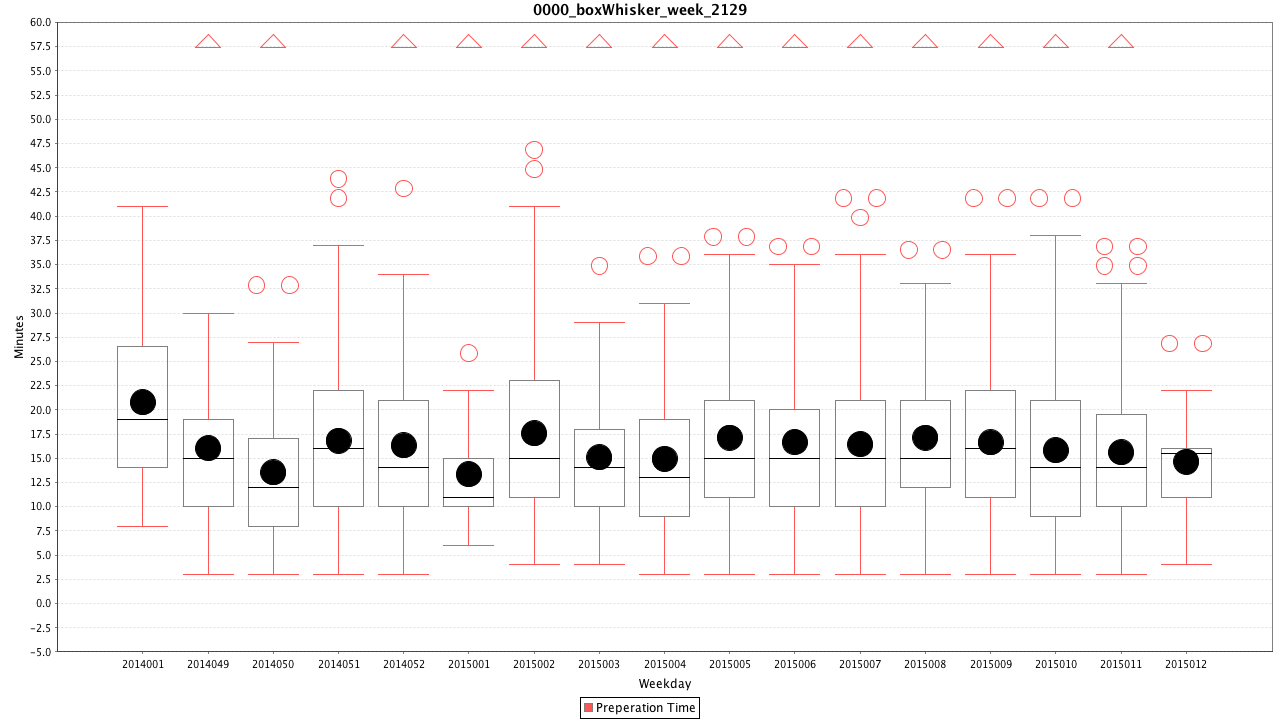
\includegraphics[width=.3\textwidth]{images/0000_boxWhisker_week_2129.png}\hfill
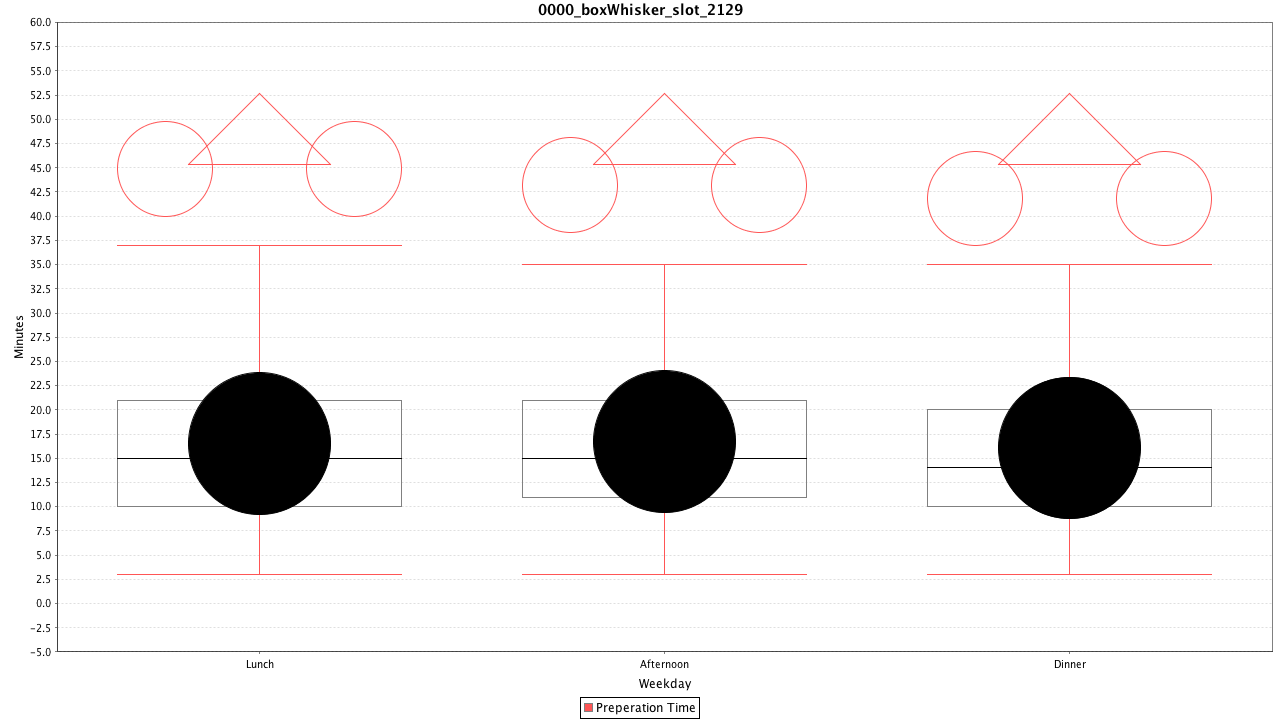
\includegraphics[width=.3\textwidth]{images/0000_boxWhisker_slot_2129.png}\hfill
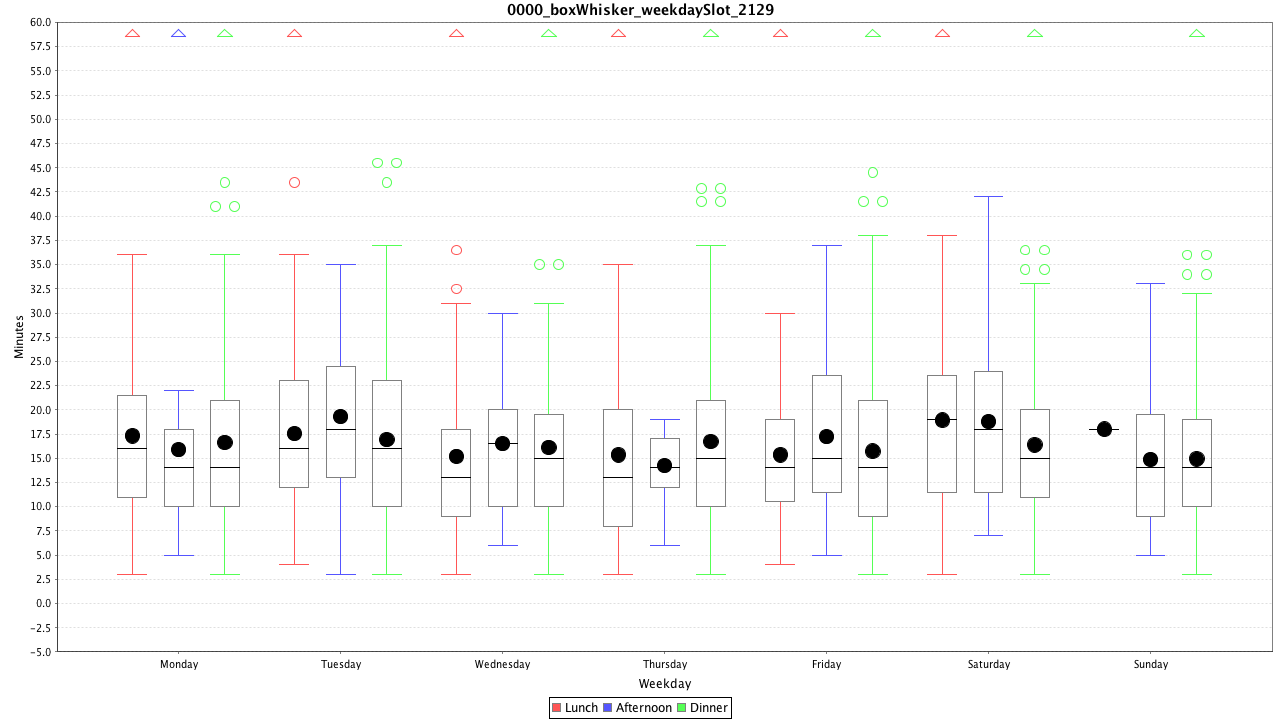
\includegraphics[width=.3\textwidth]{images/0000_boxWhisker_weekdaySlot_2129.png}

\caption{default}
\label{fig:figure3}

\end{figure}

\subsection{Restaurant Wise Proceeding}\label{subsection:Restaurant Wise Proceeding}
Before creating the model there should also be tested whether the restaurant has a significant impact on the preparation time. Restaurants are very different from each other. There are restaurants, which have already pre-cooked ingredients, others have a very simple way of preparing the meal, like sandwiches, and others are crowded at a certain time and will take longer. A pizzeria has other preparation times than a burrito take away. In order to get the best forecast possible for each restaurant they have to be looked at separately. For this purpose a popular restaurant should be chosen because it has the the largest amount of orders and is thus a good representation.
The restaurant with the most orders in the database is yum2take. yum2take is a thai take-away and restaurant and the first restaurant volo delivered from. It is also close to the office which results in a bigger number of the driver being too early than being too late. Being early has the average that it does not falsifies our data as being late does, since we do not know how long the food was already prepared. In order to get a first look at the data, a diagram categorized by slot for each weekday is created [].
\begin{figure}[h]
\begin{center}
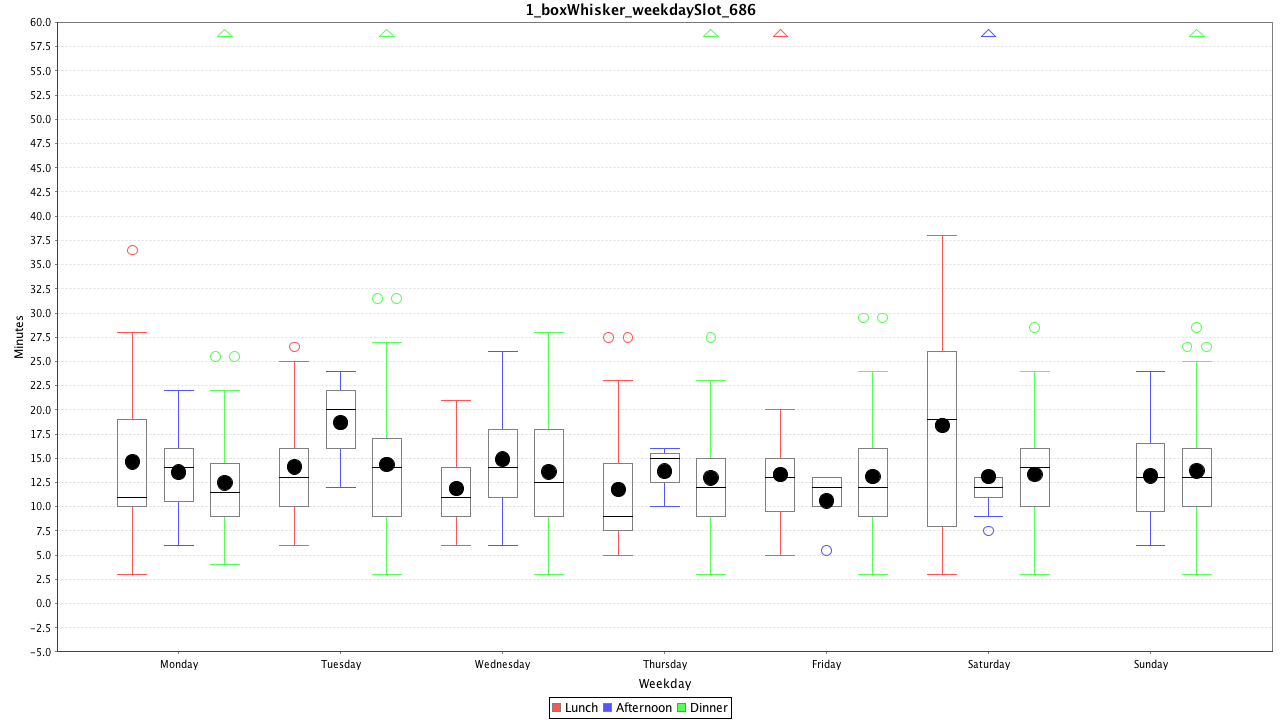
\includegraphics[width=10cm]{images/1_boxWhisker_weekdaySlot_686.png}
\caption{An example figure}
\label{fig:example}
\end{center}
\end{figure}
The distribution in the diagram for yum2take is clearly different from the overall visualization. This consolidates the assumption that restaurants should be looked at separately. The average times also have been different. For the raw data 10.2 minutes are the average, when cleaning the data from invalid values it increased to 13.5 minutes and without the outliers it lowered to 13.1 minutes.
\section{Choosing and Fitting Models}\label{section:Preliminary Analysis}
\subsection{Categorizing of Orders}\label{subsection:Categorizing by Order}
With these different first insights the model can be created. Now forecasting algorithms can be applied to the data. These are the moving average, weighted and unweighted, as well as simple exponential smoothing with different factors. They are applied to the time series of data which is free from corrupted data and outliers. As described above, this is done in Java since it can be easily integrated with the backend of volo.
In order to integrate these algorithms into Java code, the csv file had to be parsed first. This was done using a csv library. After reading the csv the raw data was processed to the diagrams seen in the preliminary analysis. The data for the models was freed from invalid entries and outliers. Then the orders were put into a map hashed by restaurant and each restaurant contained a list of orders in chronic order. For each restaurant the list of orders is passed to the forecasting unit where the calculations are done. The mean square error is calculated for the moving average and simple exponential smoothing. In order to get the best forecast, different categories are calculated.
\newline\newline\textbf{No time categorization}\newline
First of all, no time categorization is done. The forecast is done as all predecessing orders are relevant to the current one. This gives a rough estimation over the forecasting possibilities. It is not very accurate since the more orders are already included the closer the forecast is to the average. The next forecast is done with the same assumption but for each slot. Each order in the slot is forecast by all orders in that slot before it. This can eliminate the difference in case preparation times vary between the different slots. In the end the mean of the three mean square errors is taken and the root is calculated as overall root mean square error.
\newline\newline\textbf{No time but slot categorization}\newline
\newline\newline\textbf{Day categorization}\newline
After doing uncategorized forecasts, a time component is introduced. Since preparation times can vary from day to day, e.g. weekdays or holidays, they should be independent. For this reason, orders are separated by day and forecast according to this time constraint. Forecast is then done for each day as well as each slot for each day. In the end the errors of each forecast model are summed up and the average is returned. In case of the slots of each day, the average is first calculated for each slot day by day and in the end the mean errors of each slot are summed up.
\newline\newline\textbf{Day and slot categorization}\newline
\newline\newline\textbf{Week categorization}\newline
The next time categorization is on weekly basis. Like in the daily calculation, the error for each order by taking all predecessing orders of the week. This is also done for orders in a slot of each week similar to the day basis.
\newline\newline\textbf{Week and slot categorization}\newline
\newline\newline\textbf{Weekday categorization}\newline
The same procedure as for day and week categorization is done for weekday as well.
\newline\newline\textbf{Weekday and slot categorization}\newline
\newline\newline\textbf{Single slot categorization}\newline
The final simple categorization is done by separating orders into their day and slot. Each slot is then treated separately (the same way as in the day only calculation). In the end the mean square error of each slot is added up and the average is rooted to get the overall root mean square error.\newline

Before the calculation can be done, the edge case of not having predecessing orders for the current order has to be resolved. Since the operations teams suggested a 15 minute basic time for preparation, this time is always taken when no forecast value can be generated for the current order.
\subsection{Combination of Categorizations}\label{subsection:Categorizing by Order}
For the next step, Sebastian Sondheimer was interviewed. He is in the business department and joined later which is the reason he was not part of the problem definition. His focus for the forecast lies on two pillars. One is the best and most useful data to increase accuracy and the other one is to keep factors in the calculation to a minimum in order to improve speed. These two factors can work against each other and thus have to be carefully adjusted. The result is the combination of six factors which weights have to evaluated. The first factor is the forecast for the current slot in which the order is. The second value is the forecast calculated from all orders of this day. This is combined with the forecast for all orders in the last 7 days as well as the forecast for the current slot of the last day. The last two factors are the forecast for this slot of this weekday of the last 4 weeks and the overall preparation forecast of this weekday for the last 4 weeks. The weights are calculated by iterating different distributions of weights for the slots for each algorithm, namely (un)-weighted moving average and simple exponential smoothings. The results have then to be evaluated in order to find the best match.

Now that the models are set, they are run and generate forecasts. In order to evaluate the results the error for each data pair, the forecast value and the real value, is calculated by [e = yi - y^i]. The error is then squared and added to the overall error which is the sum of all errors of the time series. This is the mean square error (MSE) which is then rooted into the so called root square mean error (RMSE). This RSME represents the standard deviation of the difference between the real and the predicted value. The lower this error is, the better the forecast is.

Refer to symbols or abbreviations with\\\verb+\gls{symbolname} \glstext{symbolname} \glsfirst{symbolname}+:\\
\gls{symb:N} \glstext{symb:N} \glsfirst{symb:N}\\
\gls{BA} \gls{DA} \gls{MA}

Refer to other sections with \verb+\ref{labelname}+:\\
A reference to this subsection: \ref{labelname}

Include figures with\\
\verb+\begin{figure}+\\
\verb+...+\\
\verb+\caption{An example figure}\label{fig:example}\end{figure}+

\begin{figure}[h]
\begin{center}
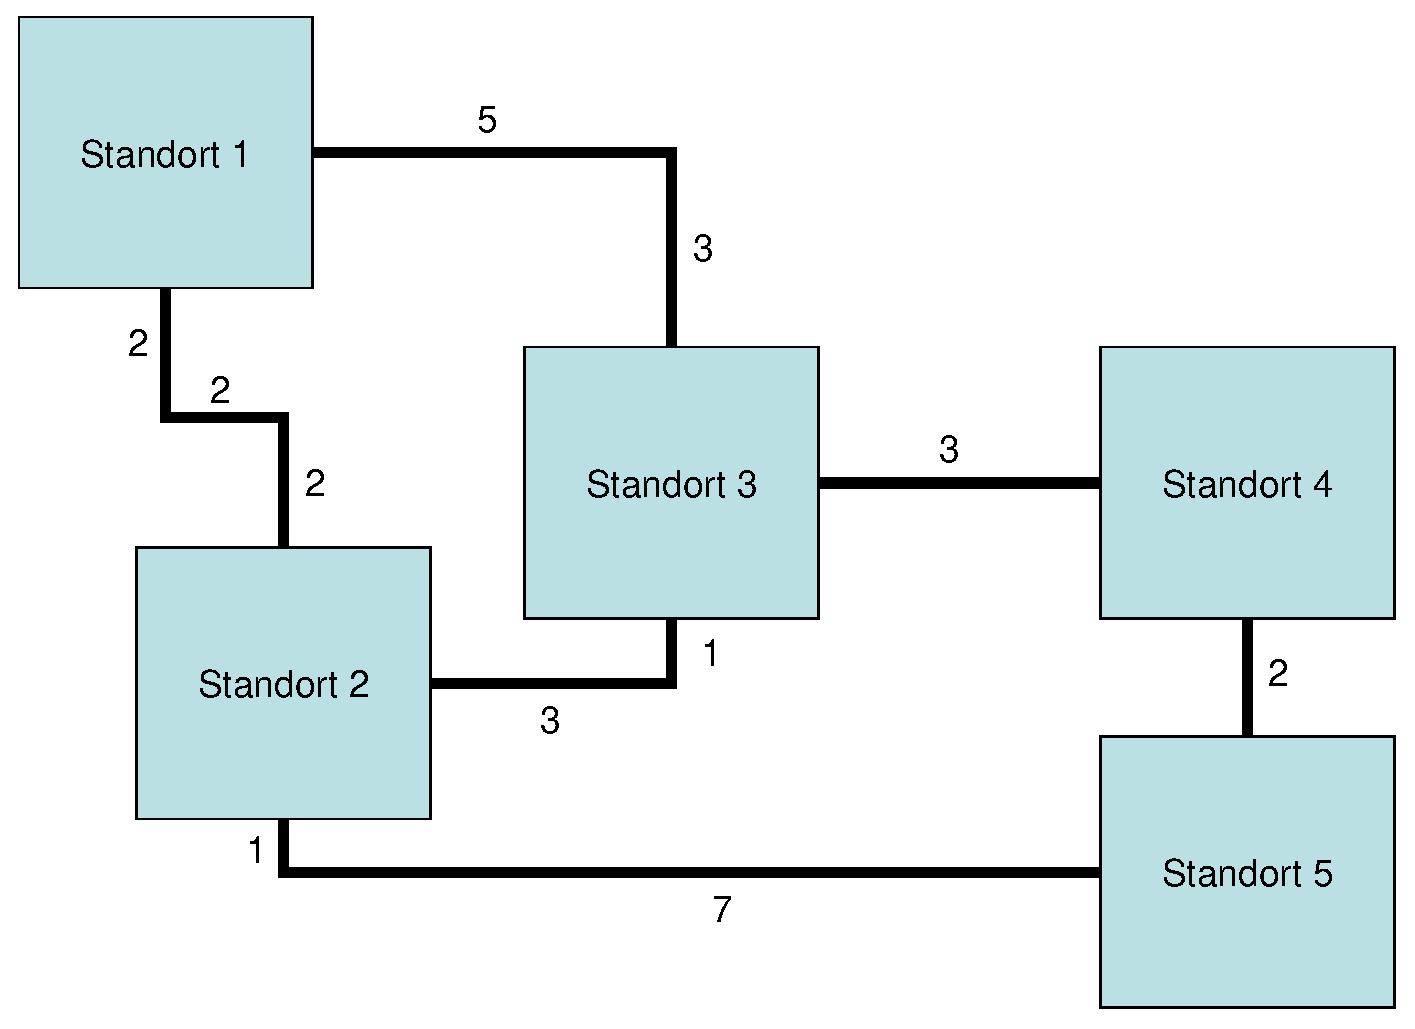
\includegraphics[width=10cm]{images/example_figure}
\caption{An example figure}
\label{fig:example}
\end{center}
\end{figure}

Include only PostScript images (.eps) if you want to create a PostScript document using dvips and only .pdf, .png, .jpeg and .gif images if your goal is a PDF document using pdflatex.
